\documentclass[10pt, compress]{beamer}

\usetheme{metropolis}
\usepackage{appendixnumberbeamer}

\usepackage{tikz-dependency}
\usepackage{caption}
\usepackage{booktabs}
\usepackage{tabularx}
\usepackage{alltt}
\usepackage[scale=2]{ccicons}

\usepackage{pgfplots}
\usepgfplotslibrary{dateplot}

\usepackage{xspace}
\newcommand{\themename}{\textbf{\textsc{metropolis}}\xspace}

% commands from the paper
\newfontfamily\gtfont[Scale=1.1,Letters=SmallCaps]{Linux Libertine O}
\newcommand{\udtag}[1]{{\ll \textsc{#1}}}
\newcommand{\gtlabel}[1]{{\gtfont #1}}
\newcommand{\udlabel}[1]{{\tt #1}}
\newfontfamily\udfont[Scale=0.9,Letters=SmallCaps]{Linux Libertine O}
\newcommand{\utag}[1]{{\udfont#1}}
\newcommand{\ufeat}[1]{{\udfont#1}}
\newcommand{\tgl}[1]{{\em #1}}
\setmonofont[Scale=MatchLowercase]{DejaVu Sans Mono}

% commands from the paper


\newcommand{\myarrow}[1][-45]{%
  \mathrel{%
    \text{$
     \begin{tikzpicture}[baseline = -0.5ex]
       \node[inner sep=0pt,outer sep=0pt,rotate = #1] (a) at (0,0)  {$\xrightarrow{}$};
    \end{tikzpicture}
    $}%
  }%
}%




\title{Class 06: Word-sense disambiguation}
\date{}
\begin{document}

\maketitle


\begin{frame}{Introduction}


\end{frame}

\begin{frame}{Context}

\begin{columns}
  \begin{column}{0.74\textwidth}
    «If one examines the words in a book, one at a time through an opaque mask 
    with a hole in it one word wide, then it is
     obviously impossible to determine, one at a 
    time, the meaning of words. ``Fast'' may mean ``rapid''; or it may mean ``motionless''; 
    and there is no way of telling which. 
    ~\\
    But, if one lengthens the slit in the opaque mask, until one can see not only 
    the central word in question but also say $N$ 
    words on either side, then, if $N$ is large 
    enough one can unambiguously decide the meaning...
    The 
    practical question is : ``What minimum value of $N$ will, at 
    least in a tolerable fraction of cases, lead to the correct choice 
    of meaning for the central word?''»
  \end{column}
  \begin{column}{0.25\textwidth}
    \begin{flushright}
    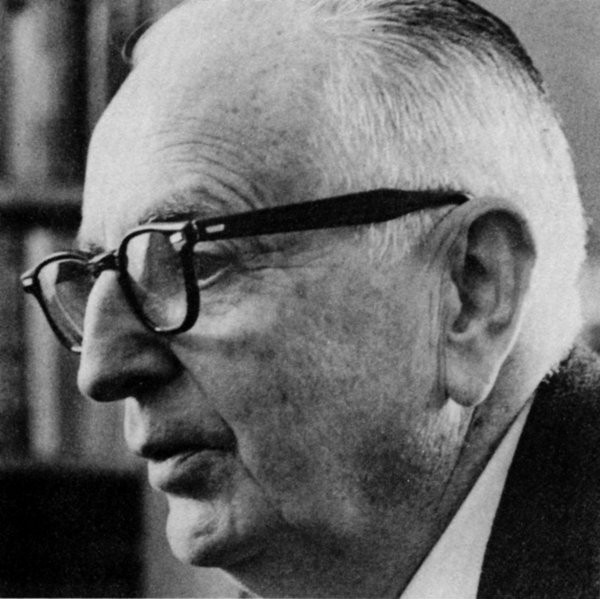
\includegraphics[width=\textwidth]{graphics/portrait-weaver-600w.jpg} \\
    Weaver (1949)
    \end{flushright}
  \end{column}
\end{columns}

\end{frame}

\begin{frame}

\begin{center}
\begin{onlyenv}<1>
\begin{tabular}{p{2.5cm}p{2.5cm}p{1.0cm}p{2.5cm}p{1.0cm}}
      &     &  \textbf{мир}  &      &      \\
      &     &  \textbf{мир}  &      &     \\
      &     &  \textbf{мир}  &      &     \\
      &     &  \textbf{мир}  &      &      \\
      &     &  \textbf{мир}  &      &      \\
      &     &  \textbf{мир}  &      &      \\
      &     &  \textbf{мир}  &      &      \\
      &     &  \textbf{мир}  &      &      \\
      &     &  \textbf{мир}  &      &      \\
      &     &  \textbf{мир}  &      &      \\
\end{tabular}
\end{onlyenv}
\begin{onlyenv}<2>
\begin{tabular}{p{2.5cm}p{2.5cm}p{1.0cm}p{2.5cm}p{1.0cm}}
      & в    &  \textbf{мир}  &      &      \\
      & России    &  \textbf{мир}  &      & \\
      & Весь    &  \textbf{мир}  &      &      \\
      & такой    &  \textbf{мир}  &      &     \\
      & заключить    &  \textbf{мир}  &      &      \\
      & виртуальный    &  \textbf{мир}  &      &      \\
      & международный    &  \textbf{мир}  &      &      \\
      & за    &  \textbf{мир}  &      &      \\
      & весь    &  \textbf{мир}  &      &      \\
      & восхваляла    &  \textbf{мир}  &      &      \\
\end{tabular}

\end{onlyenv}
\begin{onlyenv}<3>
\begin{tabular}{p{2.5cm}p{2.5cm}p{1.0cm}p{2.5cm}p{1.0cm}}
      & в    &  \textbf{мир}  &      &      \\
      & России    &  \textbf{мир}  &      & \includegraphics[width=0.35cm]{graphics/icon-dove.png} \\
      & Весь    &  \textbf{мир}  &      &  \includegraphics[width=0.35cm]{graphics/icon-world.png}    \\
      & такой    &  \textbf{мир}  &      &     \\
      & заключить    &  \textbf{мир}  &      &   \includegraphics[width=0.35cm]{graphics/icon-dove.png}   \\
      & виртуальный    &  \textbf{мир}  &      &  \includegraphics[width=0.35cm]{graphics/icon-world.png}    \\
      & международный    &  \textbf{мир}  &      & \includegraphics[width=0.35cm]{graphics/icon-dove.png}     \\
      & за    &  \textbf{мир}  &      &      \\
      & весь    &  \textbf{мир}  &      &  \includegraphics[width=0.35cm]{graphics/icon-world.png}    \\
      & восхваляла    &  \textbf{мир}  &      &  \includegraphics[width=0.35cm]{graphics/icon-dove.png}    \\
\end{tabular}

\end{onlyenv}

\begin{onlyenv}<4>
\begin{tabular}{p{2.5cm}p{2.5cm}p{1.0cm}p{2.5cm}p{1.0cm}}
      & в    &  \textbf{мир}  & значений     &      \\
      & России    &  \textbf{мир}  & со     &  \includegraphics[width=0.35cm]{graphics/icon-dove.png}    \\
      & Весь    &  \textbf{мир}  &  конечных    &  \includegraphics[width=0.35cm]{graphics/icon-world.png}    \\
      & такой    &  \textbf{мир}  &  не    &      \\
      & заключить    &  \textbf{мир}  & с     & \includegraphics[width=0.35cm]{graphics/icon-dove.png}     \\
      & виртуальный    &  \textbf{мир}  & игры     &  \includegraphics[width=0.35cm]{graphics/icon-world.png}    \\
      & международный    &  \textbf{мир}  & Организации     &  \includegraphics[width=0.35cm]{graphics/icon-dove.png}    \\
      & за    &  \textbf{мир}  & против     &      \\
      & весь    &  \textbf{мир}  &  бесконечными    &  \includegraphics[width=0.35cm]{graphics/icon-world.png}    \\
      & восхваляла    &  \textbf{мир}  & между     & \includegraphics[width=0.35cm]{graphics/icon-dove.png}     \\
\end{tabular}

\end{onlyenv}
\begin{onlyenv}<5>
\begin{tabular}{p{2.5cm}p{2.5cm}p{1.0cm}p{2.5cm}p{1.0cm}}
      & в    &  \textbf{мир}  & значений     &  \includegraphics[width=0.35cm]{graphics/icon-world.png}     \\
      & России    &  \textbf{мир}  & со     &   \includegraphics[width=0.35cm]{graphics/icon-dove.png}   \\
      & Весь    &  \textbf{мир}  &  конечных    & \includegraphics[width=0.35cm]{graphics/icon-world.png}      \\
      & такой    &  \textbf{мир}  &  не    &      \\
      & заключить    &  \textbf{мир}  & с     & \includegraphics[width=0.35cm]{graphics/icon-dove.png}     \\
      & виртуальный    &  \textbf{мир}  & игры     &  \includegraphics[width=0.35cm]{graphics/icon-world.png}     \\
      & международный    &  \textbf{мир}  & Организации     & \includegraphics[width=0.35cm]{graphics/icon-dove.png}     \\
      & за    &  \textbf{мир}  & против     &  \includegraphics[width=0.35cm]{graphics/icon-dove.png}    \\
      & весь    &  \textbf{мир}  &  бесконечными    &   \includegraphics[width=0.35cm]{graphics/icon-world.png}    \\
      & восхваляла    &  \textbf{мир}  & между     &  \includegraphics[width=0.35cm]{graphics/icon-dove.png}    \\
\end{tabular}

\end{onlyenv}


\begin{onlyenv}<6>
\begin{tabular}{p{2.5cm}p{2.5cm}p{1.0cm}p{2.5cm}p{1.0cm}}
включённостью  & в    &  \textbf{мир}  & значений     &   \includegraphics[width=0.35cm]{graphics/icon-world.png}     \\
Советской      & России    &  \textbf{мир}  & со     &    \includegraphics[width=0.35cm]{graphics/icon-dove.png}    \\
.      & Весь    &  \textbf{мир}  &  конечных    &    \includegraphics[width=0.35cm]{graphics/icon-world.png}    \\
—      & такой    &  \textbf{мир}  &  не    &      \\
необходимо      & заключить    &  \textbf{мир}  & с     &  \includegraphics[width=0.35cm]{graphics/icon-dove.png}      \\
Если      & виртуальный    &  \textbf{мир}  & игры     &   \includegraphics[width=0.35cm]{graphics/icon-world.png}     \\
и      & международный    &  \textbf{мир}  & Организации     &   \includegraphics[width=0.35cm]{graphics/icon-dove.png}     \\
борьбы      & за    &  \textbf{мир}  & против     &   \includegraphics[width=0.35cm]{graphics/icon-dove.png}     \\
охватывает      & весь    &  \textbf{мир}  &  бесконечными    &  \includegraphics[width=0.35cm]{graphics/icon-world.png}      \\
,      & восхваляла    &  \textbf{мир}  & между     &   \includegraphics[width=0.35cm]{graphics/icon-dove.png}     \\
\end{tabular}

\end{onlyenv}

\begin{onlyenv}<7>
\begin{tabular}{p{2.5cm}p{2.5cm}p{1.0cm}p{2.5cm}p{1.0cm}}
включённостью  & в    &  \textbf{мир}  & значений     &   \includegraphics[width=0.35cm]{graphics/icon-world.png}     \\
Советской      & России    &  \textbf{мир}  & со     &    \includegraphics[width=0.35cm]{graphics/icon-dove.png}    \\
.      & Весь    &  \textbf{мир}  &  конечных    &    \includegraphics[width=0.35cm]{graphics/icon-world.png}    \\
—      & такой    &  \textbf{мир}  &  не    &   \textbf{?}   \\
необходимо      & заключить    &  \textbf{мир}  & с     &  \includegraphics[width=0.35cm]{graphics/icon-dove.png}      \\
Если      & виртуальный    &  \textbf{мир}  & игры     &   \includegraphics[width=0.35cm]{graphics/icon-world.png}     \\
и      & международный    &  \textbf{мир}  & Организации     &   \includegraphics[width=0.35cm]{graphics/icon-dove.png}     \\
борьбы      & за    &  \textbf{мир}  & против     &   \includegraphics[width=0.35cm]{graphics/icon-dove.png}     \\
охватывает      & весь    &  \textbf{мир}  &  бесконечными    &  \includegraphics[width=0.35cm]{graphics/icon-world.png}      \\
,      & восхваляла    &  \textbf{мир}  & между     &   \includegraphics[width=0.35cm]{graphics/icon-dove.png}     \\
\end{tabular}

\end{onlyenv}





\end{center}
% 
% W	  — работает с речью пациента, с его включённостью в  мир значений, с его субъективным становлением в я
% P	  джа В. Буллит предложил заключить Советской России  мир со всеми иными правительствами, образовавшими
% W	  олне законченное, вечное и бесконечное целое. Весь  мир конечных вещей имеет свой источник в этом абс
% W	  наш народ и русскую землю в тяжкую кабалу, — такой  мир не даст народу желанного отдыха и успокоения.
% P	  ступления в войну России было необходимо заключить  мир с Османской империей. После достижения переми
% W	  туального мира игры к реальности. Если виртуальный  мир игры не отличается графической красотой, схем
% P	  ященные Дню борьбы за права женщин и международный  мир Организации Объединённых Наций мероприятия пр
% P	  елям Англии и земного шара с «Манифестом борьбы за  мир против ядерной войны», в котором утверждал, ч
% W	-       В Скандинавии змей Ёрмунганд охватывает весь  мир бесконечными извивами океанских глубин. Змея 
% P	  й этический характер, осуждала насилие, восхваляла  мир между людьми, честность и созидательный труд,


\end{frame}

\begin{frame}[standout]
 
Supervised word-sense disambiguation
 
\end{frame}

\begin{frame}{Word senses}

%\begin{block}
%\begin{center}
%{\Large \textbf{замок}}
%\end{center}
%\end{block}
%
%\begin{block}
%fff
%\end{block}
  
\end{frame}

% supervised wsd

%\begin{frame}{I don't believe in word senses}


% Adam Kilgarrif (1997) ”I don’t believe in word senses”. Computers and the Humanities 31 (2), pp 91–113.
%\end{frame}



% lesk algorithm


% evaluation - upper bound = human judgement

% lower bound = most-frequent sense baseline








\end{document}
